The aim of this part is to demonstrate the followoing statement

\begin{thm}
There is a measurable conjugacy $F$ between the earthquake flow $(\lambda , X) \mapsto (\lambda, E_{t \lambda}(X))$ on $\mathcal{ML}\times \mathcal{T}_g $ and the Teichmüller unipotent flow action of \[
u_t = \begin{pmatrix} 1 & t \\ 0 & 1 \end{pmatrix}
\]
on the bundle $\mathcal{QD}$ of nonzero quadratic differentials over Teichmüller space $\mathcal{T}_g$ .
\end{thm}

\[
\xymatrix{
  \mathcal{ML}\times \mathcal{T}_g  \ar[r]^{E_t} \ar[d]_F  & \mathcal{ML}\times \mathcal{T}_g \ar[d]^F \\
   \mathcal{QD} \ar[r]_{u_t} & \mathcal{QD}
 }
\]

\subsection{Tightening map}%TODO vériphier l'orthographe

A first coresspondance, found by Thurston, exist between measured foliation and measured lamination. We will mostly follow the paper of Levitt \ref{levittfoliations}.

\begin{dfnt}
We say that two foliations are equivalent if we can pass from one to the other by Whithead moves or isotopy (homeomorphism isotopic to the identity).
\end{dfnt}
\begin{center}
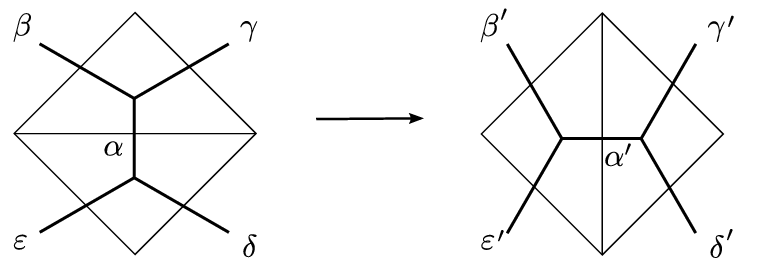
\includegraphics[width=10cm]{Image/WhiteheadMove.png}
\end{center}
%TODO définir Whithead move et une image

\begin{thm}
Let $X$ be a closed orientable hyperbolic surface and $\mathcal{F}$ a foliation. There is a canonical geodesic lamination $\gamma(\mathcal{F})$ associated to $\mathcal{F}$. If $\mathcal{F}$ and $\mathcal{F}'$ are associated foliation then $\gamma(\mathcal{F})= \gamma(\mathcal{F}')$. In the opposite direction given a geodisic lamination $\gamma$, one can find a foliation $\mathcal{F}$ such that $\gamma(\mathcal{F})=\gamma$ and it's unique up to equivalence.
\end{thm}
%TODO mettre le recouverment universel
\begin{dfnt}
A \emph{tranverse curve} is a simple closed curve $C$ which is never tangent to $\mathcal{F}$ and contain no singularity of $\mathcal{F}$.
\end{dfnt}

\begin{rmq}
Since $\mathcal{F}$ contain only saddle singularities, $C$ cannot be contractible, therefor $C$ is isotopic to a simple closed geodesic.
\end{rmq}

We will work on the universal cover of $X$, which is the Poincaré disc $\mathbb{D}$ with circle "at infinity" $\mathbb{S}$. We call $p:X \to \mathbb{D}$ the universal projection.
$\mathcal{\tilde{F}}$ is $p^{-1}(\mathcal{F})$.

We will say that a foliation follow the (*) condition if the following is true:
\begin{center}
If $f_1$ and $f_2$ are two compact homotopic leaves then all leaf in the open annulus between them  is also compact.
\end{center}

\begin{lem}
Let $h$ be a leaf of $\mathcal{\tilde{F}}$. Each end of $h$ converge to a point of $S$; the two point at infinity cannot be the same
\end{lem}

\begin{proof}
First, we should notice that the behavior of leaf at infinity do not change if we take an equivalent foliation. Indeed a homeomorphism $\phi$ on a compact fundamental domain isotopic to the identy can be extend to an homeomorphism $\tilde{\phi}$ on $\mathbb{D}$ such that $dist(x,\tilde{\phi}(x)) \leq K$. This implie that $\tilde{\phi}$ extend es the identity on the boundary $\mathbb{S}$.

\smallbreak
Then given a leaf $h$ of $\mathcal{\tilde{F}}$, we take a half leah $h_0$. If $p(h_0)$ is compact or spiral toward a compact leaf of $\mathcal{F}$ then the first part of the lemme is imediate.

\smallbreak
Otherwise, $p(h)$ meet a transverse curve $C$ infinitely often. With an isotopie we can take $C$ to be a geodesic. Now $h_0$ can meet a connect component of $\tilde{C}=p^{-1}(C)$ only one time. Otherwise there will be a disk bound by an arc of $\tilde{C}$ and an arc of $h_0$, which is impossible considering the transversity of $C$ and that $\mathcal{F}$ have no $1$-type singularities.

\smallbreak
Now every compact of $\mathbb{D}$ meet a finite number of connected components of $\tilde{C}$ so the limit set of $h_0$ must be on $\mathbb{S}$. This limit set is connected and non empty. Moreover it should not contains any end of a connected component of $\tilde{C}$. But the ends of connected components of $\tilde{C}$ are dense in $\mathbb{S}$ as $\tilde{C}$ is the image of a geodesic by $\pi_1(X)$. This show the first point of the lemma.

\smallbreak
The second assertion is clear if $p(h)$ is compact or if it meet a transverse curve $C$ at least twice since then every connected componnents of $\tilde{C}$ separate the end of $h$.

\smallbreak
Otherwise $p(h)$ spiral toward two compact leaf $f_1$ and $f_2$. If $f_1=f_2$ and the two end point of $h$ are the same then there will be a singularity that would not be a saddle. $f_1 \neq f_2$ is impossible since $\mathcal{F}$ follow the condition (*).
\end{proof}

\smallbreak
We can now associate to every leaf $h$ a geodesic $\gamma(g)$ by joining the endpoint. Then $\tilde{\gamma(\mathcal{F})}= \cup_{h \in \mathcal{F}} \gamma(h)$ is a disjoint union of geodesic invariant by $\pi_1(X)$. We have to show that this set is closed to conclued that we have a lamination.

\begin{lem}
$\tilde{\gamma(\mathcal{F})}$ is closed in $\bar{\mathbb{D}}$
\end{lem}

\begin{proof}

Let $g_n=\gamma(h_n)$ be a sequence of geodesics in $\tilde{\gamma(\mathcal{F})}$ converging to a geodesic $g$. We want to show $g \in \tilde{\gamma(\mathcal{F})}$. We can suppose that all the $g_n$ are distinct of $g$ and are all on the same side.

\smallbreak
Let $L$ be the limit set in $\bar{\mathbb{D}}$. For all leaf $m$ in $\tilde{\mathcal{F}}$, we call $\bar{m}$ the closure of $m$
 by adding the two end point in $\mathbb{S}$. Then $L$ meet at least one connected component of $\bar{\mathbb{D}} \\ \bar{m} $. As the end points of all leaf of $\tilde{\mathcal{F}}$ is a dense subset of $\mathbb{S}$, $L$ contain a leaf $h$. Taking a half-leaf $h_0$, we want to show that the end point is the same as one of $g$.

\smallbreak
A first case is if there is a simple closed curve $C$  transverse to $\mathcal{F}$ which meet $p(h_0)$ infinitely often. If $h_0$ does not converge to the corresponding point at infinity then there would be a connected component of $p^{-1}(C)$ that contains the point of infinity of $h_0$ but does not contain the point of infiny of $h_n$ which is impossible for large $n$.

\smallbreak
A second case is if $p(h_0)$ spirals toward a compact leaf, then closed leaf close to $p(h_0)$ also spirals toward the same compact leaf. Then $h_0$ converges to one of the points at infiniy of $g$ which is a point at inifinity of $h_n$ fot $n$ large.
\smallbreak

Finally if $p(h)$ is compact then $p(h_n)$ spirals toward it for large $n$, therefore $\gamma(h)$ and $g$ have one point in common at infinity. If the second was different, by applying a transformation leaving $\gamma(h)$ invariant (but no $g$), we would separate $h$ from the leaves $h_n$, and it is a contradiction.
%TODO finir la preuve : réciproque
\end{proof}

\subsection{Correspondance between foliations and quadratic differentials}

For a quadratic differential $q$, one can define two measured foliations, the horizontal $h(q)$ and the vertical $v(q)$ corresponding in locate coordinate to $Re(z)$ and $Im(z)$. This give a map two the pair of foliation but it is not the subjectif, we should restrict ro the image.
Define $\Delta = {(\alpha,\beta):i(\alpha,\gamma)=i(\beta,\gamma)=0, \text{ for some }\gamma \in \mathcal{MF}}$. $\Delta$ contain the diagonal $(\alpha,\alpha)$ and is kind of "fat" diagonal.

\begin{lem}
For any $q \in \mathcal{QD}$, $(h(q),v(q)) \notin \Delta$
\end{lem}

\subsection{Shear Cordinate}
